\documentclass[accentcolor=tud1a,colorbacktitle,inverttitle,landscape,german,presentation,t]{tudbeamer}

% usepackages
% =============================================================
\usepackage[utf8]{inputenc}
\usepackage[russian,english]{babel}

% font
\usepackage{bm}
\usepackage{pifont}
\usepackage{mxedruli}
\usepackage{soul}

% tables
\usepackage{array}
\usepackage{colortbl}
\usepackage{tabularx}
\usepackage{multirow}
\usepackage{booktabs}

\usepackage{adjustbox} 		% rotation of content

% plotting
\usepackage{tikz}
\usepackage{pgfplots}

% boxes
\usepackage[many]{tcolorbox}

% misc
\usepackage[absolute,overlay]{textpos}

% template
% =============================================================

\setbeamertemplate{section in toc}[square]

% some simple commands
% =============================================================

\newcommand{\highlight}[1]{\textcolor{tud1a}{\textbf{#1}}}

\newcommand{\gr}{\cellcolor{lightgray}}

\newcolumntype{?}{!{\vrule width 1.5pt}}

% absolute positioning of images
\newcommand{\abspos}[4]{
	\begin{textblock}{100}(#1,#2)
		\textblockcolour{white}
      		\includegraphics[scale=#4]{#3}
    	\end{textblock}
}

% divide into left and right content
\newcommand{\divideTwo}[4]{
	\begin{minipage}{#1\textwidth}
		#2
	\end{minipage}
	\hfill
	\begin{minipage}{#3\textwidth}
		#4
	\end{minipage}
}

% probing task template
\newcommand{\probingtask}[5]{
	\footnotesize
	\begin{itemize}\setlength\itemsep{1em}
		\item \textbf{Category:} \\ #1
		\item \textbf{Description:} \\ #2
		\item \textbf{Implementation:} \\ #3
		\item \textbf{Languages:} #4
		\item \textbf{Example:} \\ #5
	\end{itemize}
}

% language template
\newcommand{\lang}[5]{
	EN 	\ifnum#1=51\textcolor{green}{\ding{51}}\else\textcolor{red}{\ding{55}}\fi~~~~
	DE 	\ifnum#2=51\textcolor{green}{\ding{51}}\else\textcolor{red}{\ding{55}}\fi~~~~
	RU 	\ifnum#3=51\textcolor{green}{\ding{51}}\else\textcolor{red}{\ding{55}}\fi~~~~
	TR 	\ifnum#4=51\textcolor{green}{\ding{51}}\else\textcolor{red}{\ding{55}}\fi~~~~
	KA 	\ifnum#5=51\textcolor{green}{\ding{51}}\else\textcolor{red}{\ding{55}}\fi
}

% rotated cell content
\newcolumntype{R}[2]{%
    >{\adjustbox{angle=#1,lap=\width-(#2)}\bgroup}%
    l%
    <{\egroup}%
}
\newcommand*\rot{\multicolumn{1}{R{90}{1em}}}
\newcommand*\rotff{\multicolumn{1}{R{45}{1em}}}

% red star
\newcommand{\rs}{\textcolor{red}{\textbf{*}}}

% divider page
\newcommand{\divider}[1]{
	{\begin{frame}[plain]
		\vfill\centering
		\begin{tcolorbox}[width=4in,interior hidden,boxsep=5pt,left=0pt,right=0pt,top=2mm,
			bottom=2mm,sharp corners,colback=tud1a!40,colframe=tud1a]%%
			\centering
			\textbf{Section:} \\
			\Large \textbf{#1}
		\end{tcolorbox}
		\vfill
		\centering
		
\includegraphics[scale=0.8]{tud_logo}
		\vfill
	\end{frame}}
}

% text align
\newcommand\textalign[2][]{%
	\ifx#1l\relax
  		\makebox[0pt][l]{#2}%
	\else
  		\ifx#1r\relax
    			\makebox[0pt][r]{#2}%
  		\else  
    			\ifx#1c\relax
      				\makebox[0pt][c]{#2}%
    	\fi\fi\fi
}

% centered X column
\newcolumntype{Y}{>{\centering\arraybackslash}X}



% begin of document
% =============================================================
\begin{document}

% general information about presentation
\title[]{Interpretability of sentence embeddings in low-resource languages}
\subtitle{Mid-term presentation; \today}

\author{Daniel Wehner}
\institute[TUD UKP]{Ubiquitous Knowledge Processing, TU Darmstadt}
\logo{\color{tudtextaccent}\large UKP}
\date{\today}

\begin{titleframe}
\end{titleframe}


% Agenda
\begin{frame}{Agenda}{}
	\tableofcontents
\end{frame}


% Section: Introduction
\section{Introduction}
\divider{Introduction}


% Introduction
\begin{frame}{Introduction}{}
	\vspace*{-4mm}
	\begin{itemize}\setlength\itemsep{1em}
		\item Sentence embeddings are vectorial representations of sentences.
		\item They can be fed into ML classifiers.
		\item They have become an \textbf{integral part} in NLP applications.
		\begin{itemize}
			\item Boosted downstream task performance.
			\item Plethora of algorithms like \textit{InferSent}, \textit{sent2vec}, \textit{Quickthought}, and many more!
		\end{itemize}
		\item Neural networks are often used to obtain such embeddings.
		\item \textcolor{red}{\textbf{Problem:} Neural networks are black-box models!}
		\item Workshops like \textbf{BlackBoxNLP} attempt to \\
			shed light onto this and open the black-box.
	\end{itemize}

	\abspos{10.5}{11.5}{images/black_box}{0.2}
\end{frame}


% Interpretability of Sentence Embeddings
\begin{frame}{Interpretability of Sentence Embeddings}{}
	\vspace*{-4mm}
	\begin{itemize}\setlength\itemsep{1em}
		\item It is advantageous to know what is captured by an embedding.
		\begin{itemize}
			\item Relevant for the choice of an embedding technique for a specific task.
			\item Allows for a quality assessment of sentence embeddings.
		\end{itemize}
		\item Many authors (Shi.2016, Adi.2017, Conneau.2018; inter alia) introduce the notion of \textbf{probing tasks}.
		\item What are probing tasks?
	\end{itemize}

	\vspace*{3mm}
	\divideTwo{0.19}{
		\centering
		
\includegraphics[scale=0.2]{images/probing}
	}{0.79}{
		\begin{itemize}\setlength\itemsep{1em}
			\item Simple classification tasks that probe an embedding for \textbf{linguistic properties}.
			\item Mostly restricted to the English language in the literature.
		\end{itemize}
	}
\end{frame}


% Scope of this Thesis
\begin{frame}{Scope of this Thesis}{}
	\vspace*{-4mm}
	\begin{itemize}\setlength\itemsep{1em}
		\item The focus in this thesis is on \textbf{lower-resource languages}.
		\item Languages considered:

		\vspace*{2mm}
		{\small
		\begin{tabbing}
			\hspace*{3.5cm}\=\hspace*{3.5cm}\=\kill
			\textbf{English (EN)} 		\>											\>					\\
			\textbf{German (DE)}		\> Deutsch 									\> 					\\
			\textbf{Russian (RU)} 		\> \foreignlanguage{russian}{русский язык} 	\>	low-resource 	\\
			\textbf{Turkish (TR)} 		\> Türkçe 									\> 	low-resource 	\\
			\textbf{Georgian (KA)}	\> {\mxedr{kartuli ena}} 						\> 	low-resource
		\end{tabbing}}
		
		\item Process:
		\begin{figure}
			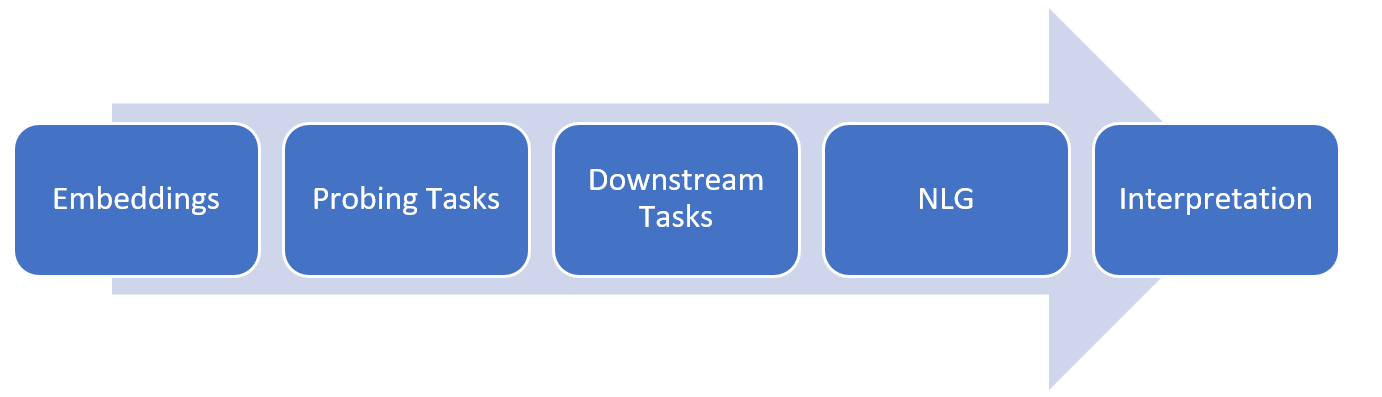
\includegraphics[scale=0.2]{images/thesis_process}
		\end{figure}
	\end{itemize}
\end{frame}


% Current Status
\begin{frame}{Current Status}{}
	\vspace*{-9mm}
	\small
	\begin{center}\parbox{0cm}{
	\begin{tabbing}
		\hspace*{1cm}\=\hspace{5cm}\= \kill
		\textbf{Item} 				\>								\>	\textalign[c]{\textbf{Status}}					\\
		Literature review 				\>								\>	\textalign[c]{\textcolor{orange}{$\bullet$}}		\\
		Implementation of... 			\>								\> 												\\
									\>	...word embeddings			\> 	\textalign[c]{\textcolor{green}{\checkmark}} 	\\
									\>	...sentence embeddings	 	\> 	\textalign[c]{\textcolor{green}{\checkmark}}	\\
									\> 	...probing tasks	 			\> 	\textalign[c]{\textcolor{green}{\checkmark}} 	\\
									\>	...downstream tasks 			\> 	\textalign[c]{\textcolor{green}{\checkmark}} 	\\
		Training of... 				\>								\> 												\\
									\> 	...word embeddings	 		\> 	\textalign[c]{\textcolor{green}{\checkmark}} 	\\
									\>	...sentence embeddings 		\> 	\textalign[c]{\textcolor{green}{\checkmark}} 	\\
		Translation of resources
									\> 								\> 	\textalign[c]{\textcolor{orange}{$\bullet$}} 		\\
		Natural language generation 	\>								\> 	\textalign[c]{\textcolor{red}{$\bm{\times}$}} 	\\
		Interpretation of results		\> 								\>	\textalign[c]{\textcolor{orange}{$\bullet$}} 		\\
		Writing thesis				\> 								\> 	\textalign[c]{\textcolor{orange}{$\bullet$}}
	\end{tabbing}}
	\end{center}
	\textbf{Legend:}~~~~ \textcolor{green}{\checkmark} done~~~~~~ \textcolor{orange}{$\bullet$} in progress~~~~~~
						\textcolor{red}{$\bm{\times}$} not started
\end{frame}


% Section: Embedding Algorithms
\section{Embedding Algorithms}
\divider{Embedding Algorithms}


% Sentence Embedding Algorithms
\begin{frame}{Sentence Embedding Algorithms}{}
	\vspace*{-4mm}
	\begin{itemize}\setlength\itemsep{1em}
		\item Two types (Yang.2018):
		\begin{itemize}
			\item \textbf{Non-parametric:} No training required, average of word embeddings.
			\item \textbf{Parametric:} Sentence embeddings are trained from scratch.
		\end{itemize}
		\item Selected algorithms for the experiments:
	\end{itemize}
	
	\hspace*{6mm}
	{\footnotesize
	\divideTwo{0.49}{
		\begin{itemize}
			\item Bag of vectors (vanilla average; 300\,d)
			\item $p$-means ($p \in \{1, 2, 3, -\infty, +\infty\}$; 1,500\,d)
			\item Geometric embeddings (GEM; 300\,d)
			\item Smooth inverse frequency (SIF; 300\,d)
			\item Hierarchical pooling (300\,d)
			\item Random embeddings (4,096 / 8,192\,d)
		\end{itemize}
	}{0.39}{
		\begin{itemize}
			\item InferSent (2,048\,d)
			\item Quickthought (2,400\,d)
			\item sent2vec (700\,d)
			\item LASER (1,024\,d)
			\item BERT (768\,d)
		\end{itemize}
	}}

	\begin{textblock*}{4cm}(1.5cm,8cm)
		\textblockcolour{tud1a!40}
		\vspace*{1mm}
		\centering
   		\textbf{Non-parametric} \strut
		\vspace*{1mm}
	\end{textblock*}

	\begin{textblock*}{4cm}(8cm,8cm)
		\textblockcolour{tud1a!40}
		\vspace*{1mm}
		\centering
   		\textbf{Parametric} \strut
		\vspace*{1mm}
	\end{textblock*}
\end{frame}


% Training Details
\begin{frame}{Training Details}{}
	\vspace*{-4mm}
	\begin{itemize}\setlength\itemsep{1em}
		\item English pre-trained models were already available for download.
		\item Other languages:
		\begin{itemize}
			\item Trained word2vec on respective Wikipedia dumps (CBoW, window size 10).
			\item Fasttext and attract-repel embeddings available for all languages.
			\item InferSent requires translation of SNLI for all languages.
			\item Quickthought / sent2vec are trained on sentences extracted from Wikipedia.
			\item LASER / BERT: Multi-lingual models are already available.
		\end{itemize}
		\item \textcolor{red}{Google translate API limits the number of translations per day. \\
			$\Rightarrow$ \textbf{The translation process is slow!} \\[3mm]
			$\approx$ 10,000 sentences / day.}
	\end{itemize}
	\abspos{10}{11.5}{images/snail}{0.3}
\end{frame}


% Section: Probing Tasks
\section{Probing Tasks}
\divider{Probing Tasks}


% Probing Tasks
\begin{frame}{Probing Tasks}{}
	\vspace*{-4mm}
	\begin{itemize}\setlength\itemsep{1em}
		\item Conneau.2018 distinguishes between three types of probing tasks: \\
			\textbf{Surface}, \textbf{Syntax} and \textbf{Semantics}
		\item Possible probing tasks (many more in the literature):
		\vspace*{2mm}
		{\footnotesize
		\begin{tabbing}
			\hspace*{3.5cm}\=\hspace*{4.5cm}\=\kill
			\ding{182}\ \textbf{Surface} 		\> 
			\ding{183}\ \textbf{Syntax} 		\>
			\ding{184}\ \textbf{Semantics} 	\\
																							\\
			Sentence length\rs 	\>	Bi-gram shift\rs 				\>	End of sentence\rs		\\
			Word content\rs 		\>	Subject-verb agreement\rs		\> 	Grammaticality 			\\
			...					\>	Subject-verb distance\rs		\> 	Object number 			\\
								\> 	Top constituent\rs 			\>	Subject number			\\
								\> 	Tree depth					\>	Tense					\\
								\> 	Voice\rs						\> 	...						\\
								\> 	Word order\rs 				\>							\\
								\> 	...							\>							\\
			{\scriptsize \rs\ $\widehat{=}$ implemented}
	\end{tabbing}}
	
	\item Limited the number of instances to 10,000.
	\end{itemize}
\end{frame}


% Probing Task: Sentence Length
\begin{frame}{Probing Task: Sentence Length}{}
	\probingtask{
		Surface probing task.
	}{
		Given a sentence embedding predict the lengths of the original sentence.
	}{
		The probing task is phrased as a 10-way classification task. The bins are as follows: \\
		{[1;4], [5;8], [9;12], [13-16], [17;20], [21;25], [26;29], [30;33], [34;55], [56;)}
	}{
		\lang{51}{51}{51}{51}{51}
	}{
		The fox jumped over the lazy dog . $\Rightarrow$ Class 1 [5;8] 
	}
	\abspos{13.5}{4.5}{images/img_sent_len}{0.2}
\end{frame}


% Probing Task: Subject-Verb Agreement
\begin{frame}{Probing Task: Subject-Verb Agreement}{}
	\probingtask{
		Syntactic probing task.
	}{
		A classifier has to predict whether the verb form agrees with the form required by the subject of the sentence.
	}{
		The task is restricted to present tense. For each language the most common verbs and their conjugations were
		acquired. Each sentence from the corpus was tested if it contains one of the words from the list. If it contains one
		such word it is replaced by different word from the list.
	}{
		\lang{51}{51}{51}{51}{51}
	}{
		 The \underline{\smash{plane}}$_{\text{subj}}$ from London to Paris \underline{take}$_{\text{verb}}$
		 	off without any delay . $\Rightarrow$ Class $\textit{`Disagree'}$
	}
	\abspos{13}{4}{images/img_sv_agree}{0.2}
\end{frame}


% Probing Task: End of Sentence
\begin{frame}{Probing Task: End of Sentence}{}
	\probingtask{
		Semantic probing task.
	}{
		Decide where a sequence of words has to be split (end of one sentence, begin of another).
	}{
		Two sentences were concatenated with punctuation removed. Also, the words were lower-cased (except for German)
		in order not to provide any hints. The possible split indices were again binned.
	}{
		\lang{51}{51}{51}{51}{51}
	}{
		 this is great $\Vert$ where are you
	}
	\abspos{13.3}{4.3}{images/img_eos}{0.2}
\end{frame}


% Section: Downstream Applications
\section{Downstream Applications}
\divider{Downstream Applications}


% Downstream Applications
\begin{frame}{Downstream Applications}{}
	\vspace*{-4mm}
	\begin{itemize}\setlength\itemsep{1em}
		\item Downstream applications considered:
		\begin{itemize}
			\item \textbf{Argumentation mining} (Labels: \texttt{FOR}, \texttt{AGAINST}, \texttt{NONE})
			\item \textbf{Sentiment analysis} (Labels: \texttt{POS}, \texttt{NEG}, \texttt{NEU})
			\item (Natural language inference)
		\end{itemize}
		\item Data sets:
		\begin{itemize}
			\item Argumentation mining:
			\begin{itemize}
				\item Data set contains $\approx$ 25,000 sentences.
				\item Various topics: abortion, nuclear energy, gun control, marijuana legalization, ...
				\item Has to be translated into all target languages. \textcolor{green}{\ding{51}}
			\end{itemize}
			\item Sentiment analysis:
			\begin{itemize}
				\item Different data set for each language.
				\item Created own data set for Georgian (since none could be found).
			\end{itemize}
		\end{itemize}
	\end{itemize}

	\abspos{12.35}{4}{images/img_arg_min}{0.25}
	\abspos{12}{7}{images/img_sentiment}{0.25}
\end{frame}


% Section: Results
\section{Results}
\divider{Results}


% Probing Task Classifier
\begin{frame}{Probing Task Classifier}{}
	\vspace*{-4mm}
	\begin{itemize}\setlength\itemsep{1em}
		\item The classifier is a Multi-Layer-Perceptron (MLP).
		\item MLP architecture:
		\begin{center}\parbox{0cm}{\begin{tabbing}
			\hspace*{5.5cm}\=\kill
			\textbf{\# hidden layers:} 				\>	1 			\\[1mm]
			\textbf{\# hidden units:} 				\> 	300 		\\[1mm]
			\textbf{Hidden layer activation func.:}	\>  	ReLU		\\[1mm]
			\textbf{Dropout rate:}					\> 	0.50 		\\[1mm]
			\textbf{\# epochs:} 					\>	30 			\\[1mm]
			\textbf{Optimizer:} 					\> 	RmsProp	\\[1mm]
			\textbf{Loss function:} 				\> Categorical cross-entropy
		\end{tabbing}}
		\end{center}
		\item Later experiments will also be conducted without the hidden layer.
	\end{itemize}
\end{frame}


% Bar Charts
\begin{frame}[plain]{}{}
	\begin{tikzpicture}
	\begin{axis}[
		scale=0.7,
		ybar,
		ylabel=Accuracy,
		enlargelimits=0.15,
		bar width=4pt,
		ymajorgrids,
    		grid style={line width=.1pt, draw=gray!10},
    		title=\textbf{Results Sentence Length Task},
		symbolic x coords={majority,p-means,laser,s2v,quickth.},
		xtick=data,
		scale only axis=true,
  		width=14cm,height=2cm,
		xticklabels={,,},
		xtick style={draw=none}
	]

		% english
		\addplot[ybar,fill=tud2a] coordinates {
			(majority,17.900)
        		(p-means,60.091)
        		(laser,71.090)
        		(s2v,32.490)
			(quickth.,71.379)
    		};

		% german
		\addplot[ybar,fill=tud1a] coordinates {
			(majority,19.900)
        		(p-means,59.311)
        		(laser,67.690)
        		(s2v,37.480)
			(quickth.,62.721)
    		};

		% russian
		\addplot[ybar,fill=tud1a!50] coordinates {
			(majority,17.400)
        		(p-means,60.240)
        		(laser,69.580)
        		(s2v,36.050)
			(quickth.,33.937)
    		};

		% turkish
		\addplot[ybar,fill=gray] coordinates {
			(majority,43.000)
        		(p-means,76.227)
        		(laser,78.729)
        		(s2v,47.545)
			(quickth.,72.845)
    		};

		% georgian
		\addplot[ybar,fill=white] coordinates {
			(majority,21.300)
        		(p-means,58.890)
        		(laser,76.450)
        		(s2v,39.920)
			(quickth.,59.860)
    		};

	\end{axis}
\end{tikzpicture}
	\begin{tikzpicture}
	\begin{axis}[
		scale=0.7,
		ybar,
		ylabel=Accuracy,
		enlargelimits=0.15,
		bar width=4pt,
		ymajorgrids,
    		grid style={line width=.1pt, draw=gray!10},
    		title=\textbf{Results Subject-Verb Agreement Task},
		symbolic x coords={majority,p-means,laser,s2v,quickth.},
		xtick=data,
		scale only axis=true,
  		width=14cm,height=2cm,
		xticklabels={,,},
		xtick style={draw=none}
	]

		% english
		\addplot[ybar,fill=tud2a] coordinates {
			(majority,54.400)
        		(p-means,64.801)
        		(laser,55.760)
        		(s2v,67.773)
			(quickth.,67.026)
    		};

		% german
		\addplot[ybar,fill=tud1a] coordinates {
			(majority,50.900)
        		(p-means,74.719)
        		(laser,59.362)
        		(s2v,76.109)
			(quickth.,80.117)
    		};

		% russian
		\addplot[ybar,fill=tud1a!50] coordinates {
			(majority,50.000)
        		(p-means,65.416)
        		(laser,72.240)
        		(s2v,77.053)
			(quickth.,75.738)
    		};

		% turkish
		\addplot[ybar,fill=gray] coordinates {
			(majority,51.400)
        		(p-means,51.407)
        		(laser,53.439)
        		(s2v,53.703)
			(quickth.,59.583)
    		};

		% georgian
		\addplot[ybar,fill=white] coordinates {
			(majority,50.400)
        		(p-means,62.206)
        		(laser,55.824)
        		(s2v,62.040)
			(quickth.,57.622)
    		};

	\end{axis}
\end{tikzpicture}
	\begin{tikzpicture}
	\begin{axis}[
		scale=0.7,
		ybar,
		ylabel=Accuracy,
		enlargelimits=0.15,
		bar width=4pt,
		ymajorgrids,
    		grid style={line width=.1pt, draw=gray!10},
    		title=\textbf{Results End of Sentence Task},
		symbolic x coords={majority,p-means,laser,s2v,quickth.},
		xtick=data,
		scale only axis=true,
  		width=14cm,height=2cm,
  		ymax=60
	]

		% english
		\addplot[ybar,fill=tud2a] coordinates {
			(majority,25.600)
        		(p-means,31.584)
        		(laser,36.675)
        		(s2v,27.252)
			(quickth.,28.219)
    		};

		% german
		\addplot[ybar,fill=tud1a] coordinates {
			(majority,20.000)
        		(p-means,30.004)
        		(laser,34.060)
        		(s2v,24.495)
			(quickth.,23.715)
    		};

		% russian
		\addplot[ybar,fill=tud1a!50] coordinates {
			(majority,23.600)
        		(p-means,32.324)
        		(laser,38.489)
        		(s2v,26.121)
			(quickth.,21.397)
    		};

		% turkish
		\addplot[ybar,fill=gray] coordinates {
			(majority,36.700)
        		(p-means,43.646)
        		(laser,52.031)
        		(s2v,36.081)
			(quickth.,44.749)
    		};

		% georgian
		\addplot[ybar,fill=white] coordinates {
			(majority,28.200)
        		(p-means,49.430)
        		(laser,55.450)
        		(s2v,42.880)
			(quickth.,51.420)
    		};

	\end{axis}
\end{tikzpicture}

	\begin{center}
		\textcolor{tud2a}{\ding{110}} EN~~~~
		\textcolor{tud1a}{\ding{110}} DE~~~~
		\textcolor{tud1a!50}{\ding{110}} RU~~~~
		\textcolor{gray}{\ding{110}} TR~~~~
		$\square$ KA
	\end{center}
\end{frame}


% Probing Task Results for Georgian
\begin{frame}{Probing Task Results for Georgian}{}
	\vspace*{-8mm}
	\begin{table}[h]
	\centering
	\renewcommand{\arraystretch}{1.65}
	\scalebox{0.4}{
	\begin{tabularx}{30cm}{
		| l | Y | Y | Y | Y | Y | Y | Y | Y | 
	}
	\hline
	\multicolumn{9}{| c |}{
		\cellcolor{tud1a}\textcolor{white}{
			\textbf{Language: Georgian}}} 				\\
		\cellcolor{tud1a!70}\textbf{Embedding}				& 
		\cellcolor{tud1a!70}\textbf{Sentence length} 		&
		\cellcolor{tud1a!70}\textbf{End of sentence} 		&
		\cellcolor{tud1a!70}\textbf{Word content}			&
		\cellcolor{tud1a!70}\textbf{Word order} 			&
		\cellcolor{tud1a!70}\textbf{Bi-gram shift} 			&
		\cellcolor{tud1a!70}\textbf{Voice} 					&
		\cellcolor{tud1a!70}\textbf{SV agreement}			&
		\cellcolor{tud1a!70}\textbf{SV distance}				\\
	\hline\hline
	\multicolumn{9}{| l |}{\cellcolor{tud1a!30}\textbf{Size of the data set}} \\ \hline
	\# instances &
                10,000 	&
                10,000 	&
                8,674 		&
                262		&
                10,000 	&
                10,000 	&
                7,786 		&
                n.\,i. 		\\  
	\hline\hline 
	\multicolumn{9}{| l |}{\cellcolor{tud1a!30}\textbf{Majority class (baseline)}} \\ \hline
	\rowcolor{lightgray!30}
	Majority &
                21.300 &
                28.200 &
                13.000 &
                33.500 &
                50.100 &
                69.100 &
                50.400 &
                n.\,i. \\
	\hline\hline   
	\multicolumn{9}{| l |}{\cellcolor{tud1a!30}\textbf{Random embeddings (baseline)}} \\ \hline
	\rowcolor{lightgray!30}
	BOREP &
                47.640 &
                46.000 &
                57.157 &
                33.084 &
                50.570 &
                79.390 &
                61.847 &
                n.\,i. \\
        \hline
		\rowcolor{lightgray!30}
        ESN &
                46.439 &
                43.129 &
                30.956 &
                32.309 &
                50.220 &
                76.800 &
                53.178 &
                n.\,i. \\
        \hline
		\rowcolor{lightgray!30}
        Random LSTM &
                54.450 &
                49.590 &
                45.348 &
                35.748 &
                50.460 &
                79.850 &
                59.895 &
                n.\,i. \\
	\hline\hline
	\multicolumn{9}{| l |}{\cellcolor{tud1a!30}\textbf{Average embeddings (fasttext)}} \\ \hline
	Vanilla average &
                33.400 &
                39.200 &
                64.786 &
                33.075 &
                49.630 &
                79.040 &
                \cellcolor{tud1a!70}64.415 &
                n.\,i. \\
        \hline
        p-Means &
                58.890 &
                49.430 &
                64.829 &
                33.084 &
                50.260 &
                \cellcolor{tud1a!70}81.460 &
                62.206 &
                n.\,i. \\
        \hline
        SIF &
                30.780 &
                37.610 &
                64.485 &
                32.701 &
                48.990 &
                78.260 &
                64.056 &
                n.\,i. \\
        \hline
        GEM &
                39.660 &
                43.420 &
                83.815 &
                32.692 &
                49.830 &
                79.040 &
                63.799 &
                n.\,i. \\
        \hline
        hier. pooling &
                54.870 &
                49.400 &
                55.816 &
                32.683 &
                49.710 &
                80.580 &
                62.271 &
                n.\,i. \\
	\hline\hline
	\multicolumn{9}{| l |}{\cellcolor{tud1a!30}\textbf{Trained embeddings}} \\ \hline
	InferSent &
		   \textcolor{orange}{$\bm{\triangle}$} &
		   \textcolor{orange}{$\bm{\triangle}$} &
		   \textcolor{orange}{$\bm{\triangle}$} &
		   \textcolor{orange}{$\bm{\triangle}$} &
		   \textcolor{orange}{$\bm{\triangle}$} &
		   \textcolor{orange}{$\bm{\triangle}$} &
		   \textcolor{orange}{$\bm{\triangle}$} &
                n.\,i. \\
        \hline
        QuickThought &
                59.860 &
                51.420 &
                73.707 &
                \cellcolor{tud1a!70}84.403 &
                54.300 &
                76.440 &
                57.622 &
                n.\,i. \\
        \hline
        sent2vec &
                39.920 &
                42.880 &
                \cellcolor{tud1a!70}91.711 &
                33.467 &
                50.450 &
                75.820 &
                62.040 &
                n.\,i. \\
        \hline
        BERT &
                59.789 &
                50.170 &
                54.005 &
                46.382 &
                \cellcolor{tud1a!70}57.090 &
                78.940 &
                54.604 &
                n.\,i. \\
        \hline
        LASER &
                \cellcolor{tud1a!70}76.450 &
                \cellcolor{tud1a!70}55.450 &
                40.705 &
                45.293 &
                55.630 &
                79.440 &
                55.824 &
                n.\,i. \\
	\hline
	\end{tabularx}}
\end{table}
\end{frame}


% Training Set Size matters!
\begin{frame}{Training Set Size matters!}{}
	\vspace*{-4mm}
	Example for EN:
	\begin{figure}
		\centering
		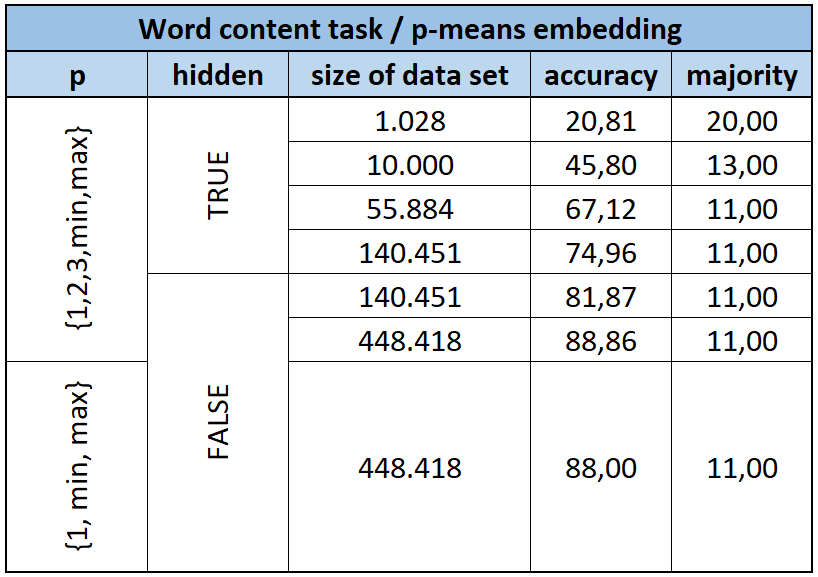
\includegraphics[scale=0.35]{images/effect_training_set_size}
	\end{figure}
\end{frame}


% Results Argumentation Mining
\begin{frame}{Results Argumentation Mining}{}
	\vspace*{-8mm}
	\begin{center}\parbox{0cm}{\begin{tabbing}
		\hspace*{3.5cm}\=\hspace*{4.5cm}\=\kill
		\textbf{Language} 	\>
		\textbf{Accuracy} 	\>
		\textbf{Embedding}	\\[3mm]
		-		\>	56.200 	\> 	Majority		\\[1mm]
		EN		\>	65.407	\>	sent2vec 	\\[1mm]
		DE		\>	65.080 	\>	LASER 		\\[1mm]
		RU		\>	63.873	\> 	LASER 		\\[1mm]
		TR		\>	64.106	\>	LASER 		\\[1mm]
		KA		\>	61.867	\>	SIF
	\end{tabbing}}
	\end{center}

	\begin{itemize}\setlength\itemsep{1em}
		\item For downstream tasks it would be better to compute F1-scores.
		\item It is not necessary to achieve state-of-the-art performance. \\
			It is more important to be able to compare embeddings given an architecture.
	\end{itemize}
\end{frame}


% Findings
\begin{frame}{Findings}{}
	\vspace*{-4mm}
	\begin{itemize}\setlength\itemsep{1em}
		\item Trained models usually perform best \\
			(except for Georgian; models might need more training data).
		\item All embeddings are above the majority baseline.
		\item High accuracy for random embeddings probably due to high dimensionality. 
		\item LASER performs well on sentence length, end of sentence, voice and subject-verb distance.
		\item s2v shows strong performance on word content, otherwise bad performance.
		\item Quickthought performs well on word order task.
		\item \textbf{Training data set size matters!}
	\end{itemize}
\end{frame}


% Section: Summary
\section{Summary}
\divider{Summary}


% Summary
\begin{frame}{Summary}{}
	\begin{itemize}\setlength\itemsep{1em}
		\item It is \textbf{not clear} what linguistic properties are captured by sentence embeddings.
		\item \textbf{Probing tasks} are an attempt to shed light onto this.
		\item Downstream applications evaluate embeddings in \textbf{real applications}.
		\item \textbf{Outlook:}
		\begin{itemize}
			\item Acquire \textbf{larger probing data sets} \\
				(especially for word content and word order task).
			\item \textbf{Interpretation of results} and comparison to literature.
			\item Implementation of \textbf{NLG}.
		\end{itemize}
	\end{itemize}
\end{frame}


% Thank you page
\begin{frame}[plain]
	\vfill\centering
	\begin{tcolorbox}[width=4in,interior hidden,boxsep=5pt,left=0pt,right=0pt,top=2mm,
		bottom=2mm,sharp corners,colback=tud1a!40,colframe=tud1a]%%
		\centering
		\Large\textbf{Thank you very much for your attention!}
	\end{tcolorbox}
	\vfill
	\begin{center}\parbox{0cm}{
	{\footnotesize
	\begin{tabbing}
		\hspace*{3.5cm}\=\kill
		\textbf{Presenter:} 	\>	Daniel Wehner \\[2mm]
		\textbf{Date:}		\>	\today \\[2mm]
		\textbf{Topic:}		\>	Interpretability of sentence embeddings \\
							\>	in low-resource languages \\
	\end{tabbing}}}
	\end{center}
	\vfill
	\centering
	
\includegraphics[scale=0.8]{tud_logo}
	\vfill
\end{frame}


% Section: Appendix
\section*{Appendix}
\divider{Appendix}

% Subsection: Further Probing Tasks
\subsection*{Further Probing Tasks}
\divider{Further Probing Tasks}


% Probing Task: Word Content
\begin{frame}{Probing Task: Word Content}{}
	\probingtask{
		Surface probing task.
	}{
		Decide which of 30 possible words is contained in the sentence.
	}{
		30 mid-frequency nouns were chosen for each language. Each sentence in the data set is chosen such that
			\textbf{exactly one} noun from the list is contained in the sentence.
	}{
		\lang{51}{51}{51}{51}{51}
	}{
		 Federal elections took place last year. $\Rightarrow$ Class \textit{`Year'}
	}
	\abspos{13}{4}{images/img_wc}{0.25}
\end{frame}


% Probing Task: Word Order
\begin{frame}{Probing Task: Word Order}{}
	\vspace*{-3mm}
	\probingtask{
		Syntactic probing task.
	}{
		Decide if a word is located at the beginning, the end or in the middle of a sentence (3-way classification).
	}{
		The most common noun in the corpus was chosen. The data set comprises sentences which contain this word
			\textbf{exactly once}. The word considered to be at the beginning/end if it is among the first/last 5 words
			in the sentence (4 for Turkish and Georgian due to agglutinative property).
	}{
		\lang{51}{51}{51}{51}{51}
	}{
		 This \underline{\smash{year}} a new software $\Vert$ update was released which patched $\Vert$ 
		 	most of the vulnerabilities . \\ $\Rightarrow$ Class \textit{`Beginning'}
	}
\end{frame}


% Probing Task: Bi-Gram Shift
\begin{frame}{Probing Task: Bi-Gram Shift}{}
	\vspace*{-3mm}
	\probingtask{
		Syntactic probing task.
	}{
		Tests for a legal word order. The classifier has to decide if a bi-gram was switched or not.
	}{
		In 50\,\% of the time a word in the sentence was picked randomly which subsequently switched positions with its
			right neighbor. In the other cases the sentences remained unaltered.
	}{
		\lang{51}{51}{51}{51}{51}
	}{
		 This is awesome . (Class 0) $\Rightarrow$ This awesome is . (Class 1)
	}
\end{frame}


% Probing Task: Voice
\begin{frame}{Probing Task: Voice}{}
	\vspace*{-3mm}
	\probingtask{
		Syntactic probing task.
	}{
		Probes a sentence embedding whether it encodes information about the voice of the sentence (active / passive).
	}{
		Sentences from the corpus containing a passive construct were labeled accordingly.
	}{
		\lang{51}{51}{51}{51}{51}
	}{
		 This picture was painted by Leonardo Da Vinci. $\Rightarrow$ Class \textit{`Passive'}
	}
\end{frame}


% Probing Task: Subject-Verb Distance
\begin{frame}{Probing Task: Subject-Verb Distance}{}
	\vspace*{-3mm}
	\probingtask{
		Syntactic probing task.
	}{
		A classifier has to predict how far subject and verb are apart.
	}{
		Similar to the sentence length task the number of words is binned. The bins were chosen as follows: 
			[1], [2;4], [5;7], [8;12], [13;).
			Given a sentence representation the classifier has to decide for a bin. The task is not implemented for Georgian
			since the corpus does not include dependency parses.
	}{
		\lang{51}{51}{51}{51}{55}
	}{
		 The \underline{\smash{plane}}$_{\text{subj}}$ from London to Paris \underline{takes}$_{\text{verb}}$
		 	off without any delay . $\Rightarrow$ Class 1 [2;4]
	}
\end{frame}


% Probing Task: Top Constituent
\begin{frame}{Probing Task: Top Constituent}{}
	\vspace*{-3mm}
	\probingtask{
		Syntactic probing task.
	}{
		Sentences are labeled with their top constituent. The task is formulated as a 10-way classification task.
	}{
		The Stanford Parser was used for English and German. For Georgian a small data set was made available.
			The 9 most frequent top constituents were taken as a label. The rest was labeled with `\texttt{Other}'.
	}{
		\lang{51}{51}{55}{55}{51}
	}{
		 The children went to school. $\Rightarrow$ \texttt{NP VP .}
	}
\end{frame}


% Sentiment Data Set for Georgian
\begin{frame}{Sentiment Data Set for Georgian}{}
	\vspace*{-4mm}
	\begin{itemize}\setlength\itemsep{1em}
		\item Collected tweets from Georgian Twitter and labeled tweets with sentiment based on emojis used
			(Choudhary.2018).
		\vspace*{2mm}
		\begin{table}[h]
	\centering
	\renewcommand{\arraystretch}{1.4}
	\scalebox{0.45}{
	\begin{tabular}{m{1cm} m{4cm} m{1cm} m{4cm} m{1cm} m{4cm}}
		\toprule
		\multicolumn{2}{c}{\textbf{Positive sentiment}} 	&
		\multicolumn{2}{c}{\textbf{Neutral sentiment}} 		&
		\multicolumn{2}{c}{\textbf{Negative sentiment}} 	\\ \cmidrule(lr){1-2} \cmidrule(lr){3-4} \cmidrule(lr){5-6}
		\textbf{Emoji} & \textbf{Short name} & \textbf{Emoji} & \textbf{Short name} & \textbf{Emoji} & \textbf{Short name}
		\\ \cmidrule(lr){1-1} \cmidrule(lr){2-2} \cmidrule(lr){3-3} \cmidrule(lr){4-4} \cmidrule(lr){5-5} \cmidrule(lr){6-6}
		\addlinespace
		
\includegraphics[scale=0.125]{images/emoji/heart_eyes.png} & \texttt{:heart\_eyes:} &
		
\includegraphics[scale=2.1]{images/emoji/no_mouth.png} & \texttt{:no\_mouth:} &
		
\includegraphics[scale=2.1]{images/emoji/cry.png} & \texttt{:cry:}
		\\
		
\includegraphics[scale=2.1]{images/emoji/grinning.png} & \texttt{:grinning:} &
		
\includegraphics[scale=0.145]{images/emoji/thinking_face.png} & \texttt{:thinking\_face:} &
		
\includegraphics[scale=2.1]{images/emoji/angry.png} & \texttt{:angry:}
		\\
		
\includegraphics[scale=0.145]{images/emoji/grin.png} & \texttt{:grin:} &
		
\includegraphics[scale=2.1]{images/emoji/neutral_face.png} & \texttt{:neutral\_face:} &
		
\includegraphics[scale=2.1]{images/emoji/rage.png} & \texttt{:rage:}
		\\
		
\includegraphics[scale=2.1]{images/emoji/joy.png} & \texttt{:joy:} &
		
\includegraphics[scale=2.1]{images/emoji/smirk.png} & \texttt{:smirk:} &
		
\includegraphics[scale=2.1]{images/emoji/sob.png} & \texttt{:sob:}
		\\
  		\bottomrule
	\end{tabular}}
\end{table}
		\item Procedure:
		\begin{enumerate}
			\item Got a list of most frequent words.
			\item Search term: One word from the list and an emoji.
			\item Non-Georgian text was filtered / hashing to prevent duplicate tweets.
			\item The data set contains around 13,000 tweets.
		\end{enumerate}
	\end{itemize}
\end{frame}


% Subsection: Detailed Results
\subsection*{Detailed Results}
\divider{Detailed Results}


% Probing Task Results for English
\begin{frame}{Probing Task Results for English}{}
	\vspace*{-8mm}
	\begin{table}[h]
	\centering
	\renewcommand{\arraystretch}{1.65}
	\scalebox{0.4}{
	\begin{tabularx}{30cm}{
		| l | Y | Y | Y | Y | Y | Y | Y | Y |
	}
	\hline
	\multicolumn{9}{| c |}{
		\cellcolor{tud1a}\textcolor{white}{
			\textbf{Language: English}}} 					\\
		\cellcolor{tud1a!70}\textbf{Embedding}				& 
		\cellcolor{tud1a!70}\textbf{Sentence length} 		&
		\cellcolor{tud1a!70}\textbf{End of sentence} 		&
		\cellcolor{tud1a!70}\textbf{Word content}			&
		\cellcolor{tud1a!70}\textbf{Word order} 			&
		\cellcolor{tud1a!70}\textbf{Bi-gram shift} 			&
		\cellcolor{tud1a!70}\textbf{Voice} 					&
		\cellcolor{tud1a!70}\textbf{SV agreement}			&
		\cellcolor{tud1a!70}\textbf{SV distance}				\\
	\hline\hline
	\multicolumn{9}{| l |}{\cellcolor{tud1a!30}\textbf{Size of the data set}} \\ \hline
	\# instances &
                9,997 		&
                5,283 		&
                1,028 		&
                557 		&
                9,997 		&
                9,997 		&
                5,485 		&
                6,045 		\\  
	\hline\hline 
	\multicolumn{9}{| l |}{\cellcolor{tud1a!30}\textbf{Majority class (baseline)}} \\ \hline
	\rowcolor{lightgray!30}
	Majority &
                17.900 &
                25.600 &
                20.500 &
                33.333 &
                50.500 &
                90.200 &
                54.400 &
                49.600 \\
	\hline\hline   
	\multicolumn{9}{| l |}{\cellcolor{tud1a!30}\textbf{Random embeddings (baseline)}} \\ \hline
	\rowcolor{lightgray!30}
	BOREP &
                44.865 &
                28.065 &
                21.004 &
                33.333 &
                50.025 &
                90.187 &
                64.036 &
                53.458 \\
        \hline
	\rowcolor{lightgray!30}
        ESN &
                42.189 &
                25.625 &
                20.512 &
                33.333 &
                50.255 &
                90.187 &
                50.747 &
                50.249 \\
        \hline
	\rowcolor{lightgray!30}
        Random LSTM &
                55.229 &
                31.224 &
                20.512 &
                33.333 &
                50.615 &
                90.427 &
                63.926 &
                57.924 \\
	\hline\hline
	\multicolumn{9}{| l |}{\cellcolor{tud1a!30}\textbf{Average embeddings (fasttext)}} \\ \hline
	Vanilla average &
                31.600 &
                26.796 &
                22.372 &
                33.333 &
                51.510 &
                91.200 &
                67.408 &
                59.726 \\
        \hline
        p-Means &
                60.091 &
                31.584 &
                20.805 &
                33.333 &
                49.800 &
                90.480 &
                64.801 &
                57.130 \\
        \hline
        SIF &
                28.300 &
                26.476 &
                21.101 &
                33.333 &
                50.620 &
                90.800 &
                65.585 &
                59.230 \\
        \hline
        GEM &
                36.530 &
                27.403 &
                59.881 &
                32.796 &
                50.550 &
                90.600 &
                60.171 &
                56.747 \\
        \hline
        hier. pooling &
                54.787 &
                30.202 &
                20.608 &
                34.229 &
                51.485 &
                89.937 &
                64.072 &
                60.669 \\
	\hline\hline
	\multicolumn{9}{| l |}{\cellcolor{tud1a!30}\textbf{Trained embeddings}} \\ \hline
	InferSent &
		   \textcolor{orange}{$\bm{\triangle}$} &
		   \textcolor{orange}{$\bm{\triangle}$} &
		   \textcolor{orange}{$\bm{\triangle}$} &
		   \textcolor{orange}{$\bm{\triangle}$} &
		   \textcolor{orange}{$\bm{\triangle}$} &
		   \textcolor{orange}{$\bm{\triangle}$} &
		   \textcolor{orange}{$\bm{\triangle}$} &
		   \textcolor{orange}{$\bm{\triangle}$} \\
        \hline
        QuickThought &
                \cellcolor{tud1a!70}71.379 &
                28.219 &
                30.110 &
                \cellcolor{tud1a!70}69.713 &
                52.660 &
                90.100 &
                67.026 &
                63.066 \\
        \hline
        sent2vec &
                32.490 &
                27.252 &
                \cellcolor{tud1a!70}62.631 &
                38.172 &
                51.570 &
                91.210 &
                \cellcolor{tud1a!70}67.773 &
                59.047 \\
        \hline
        BERT &
                53.989 &
                33.006 &
                40.812 &
                50.179 &
                \cellcolor{tud1a!70}63.920 &
                90.500 &
                62.650 &
                64.637 \\
        \hline
        LASER &
                71.090 &
                \cellcolor{tud1a!70}36.675 &
                21.099 &
                65.233 &
                58.040 &
                \cellcolor{tud1a!70}93.650 &
                55.760 &
                \cellcolor{tud1a!70}68.790 \\
	\hline
	\end{tabularx}}
\end{table}	
\end{frame}


% Probing Task Results for German
\begin{frame}{Probing Task Results for German}{}
	\vspace*{-8mm}
	\begin{table}[h]
	\centering
	\renewcommand{\arraystretch}{1.65}
	\scalebox{0.4}{
	\begin{tabularx}{30cm}{
		| l | Y | Y | Y | Y | Y | Y | Y | Y |
	}
	\hline
	\multicolumn{9}{| c |}{
		\cellcolor{tud1a}\textcolor{white}{
			\textbf{Language: German}}} 					\\
		\cellcolor{tud1a!70}\textbf{Embedding}				& 
		\cellcolor{tud1a!70}\textbf{Sentence length} 		&
		\cellcolor{tud1a!70}\textbf{End of sentence} 		&
		\cellcolor{tud1a!70}\textbf{Word content}			&
		\cellcolor{tud1a!70}\textbf{Word order} 			&
		\cellcolor{tud1a!70}\textbf{Bi-gram shift} 			&
		\cellcolor{tud1a!70}\textbf{Voice} 					&
		\cellcolor{tud1a!70}\textbf{SV agreement}			&
		\cellcolor{tud1a!70}\textbf{SV distance}				\\
	\hline\hline
	\multicolumn{9}{| l |}{\cellcolor{tud1a!30}\textbf{Size of the data set}} \\ \hline
	\# instances &
                10,000 	&
                6,708 		&
                977 		&
                766 		&
                10,000 	&
		   10,000 	&
                3,432 		&
                10,000 	\\  
	\hline\hline 
	\multicolumn{9}{| l |}{\cellcolor{tud1a!30}\textbf{Majority class (baseline)}} \\ \hline
	\rowcolor{lightgray!30}
	Majority &
                19.900 &
                20.000 &
                04.200 &
                33.400 &
                50.200 &
                80.400 &
                50.900 &
                43.600 \\
	\hline\hline   
	\multicolumn{9}{| l |}{\cellcolor{tud1a!30}\textbf{Random embeddings (baseline)}} \\ \hline
	\rowcolor{lightgray!30}
	BOREP &
                41.372 &
                23.244 &
                06.056 &
                33.377 &
                49.660 &
                82.240 &
                78.491 &
                46.320 \\
        \hline
		\rowcolor{lightgray!30}
        ESN &
                26.845 &
                18.126 &
                04.175 &
                33.377 &
                50.060 &
                80.430 &
                50.596 &
                43.600 \\
        \hline
		\rowcolor{lightgray!30}
        Random LSTM &
                56.030 &
                27.183 &
                09.699 &
                37.133 &
                50.570 &
                85.360 &
                75.357 &
                48.379 \\
	\hline\hline
	\multicolumn{9}{| l |}{\cellcolor{tud1a!30}\textbf{Average embeddings (fasttext)}} \\ \hline
	Vanilla average &
                30.220 &
                23.462 &
                20.825 &
                30.530 &
                49.070 &
                93.230 &
                77.504 &
                49.610 \\
        \hline
        p-Means &
                59.311 &
                30.004 &
                13.302 &
                33.247 &
                49.520 &
                90.020 &
                74.719 &
                46.940 \\
        \hline
        SIF &
                27.120 &
                22.517 &
                26.061 &
                27.945 &
                49.490 &
                87.500 &
                76.139 &
                47.110 \\
        \hline
        GEM &
                34.340 &
                21.515 &
                56.152 &
                23.416 &
                49.640 &
                94.450 &
                75.704 &
                47.060 \\
        \hline
        hier. pooling &
                52.150 &
                27.402 &
                16.618 &
                32.598 &
                49.890 &
                87.390 &
                74.659 &
                47.880 \\
	\hline\hline
	\multicolumn{9}{| l |}{\cellcolor{tud1a!30}\textbf{Trained embeddings}} \\ \hline
	InferSent &
		   \textcolor{orange}{$\bm{\triangle}$} &
		   \textcolor{orange}{$\bm{\triangle}$} &
		   \textcolor{orange}{$\bm{\triangle}$} &
		   \textcolor{orange}{$\bm{\triangle}$} &
		   \textcolor{orange}{$\bm{\triangle}$} &
		   \textcolor{orange}{$\bm{\triangle}$} &
		   \textcolor{orange}{$\bm{\triangle}$} &
		   \textcolor{orange}{$\bm{\triangle}$} \\
        \hline
        QuickThought &
                62.721 &
                23.715 &
                22.566 &
                39.198 &
                58.840 &
                \cellcolor{tud1a!70}94.570 &
                \cellcolor{tud1a!70}80.117 &
                \cellcolor{tud1a!70}58.341 \\
        \hline
        sent2vec &
                37.480 &
                24.495 &
                \cellcolor{tud1a!70}88.854 &
                24.711 &
                51.290 &
                93.630 &
                76.109 &
                50.320 \\
        \hline
        BERT &
                49.849 &
                29.641 &
                39.288 &
                \cellcolor{tud1a!70}42.945 &
                \cellcolor{tud1a!70}63.910 &
                88.780 &
                72.830 &
                52.280 \\
        \hline
        LASER &
                \cellcolor{tud1a!70}67.690 &
                \cellcolor{tud1a!70}34.060 &
                28.300 &
                41.145 &
                58.460 &
                90.660 &
                59.362 &
                55.750 \\
	\hline
	\end{tabularx}}
\end{table}	
\end{frame}


% Probing Task Results for Russian
\begin{frame}{Probing Task Results for Russian}{}
	\vspace*{-8mm}
	\begin{table}[h]
	\centering
	\renewcommand{\arraystretch}{1.65}
	\scalebox{0.4}{
	\begin{tabularx}{30cm}{
		| l | Y | Y | Y | Y | Y | Y | Y | Y |
	}
	\hline
	\multicolumn{9}{| c |}{
		\cellcolor{tud1a}\textcolor{white}{
			\textbf{Language: Russian}}} 					\\
		\cellcolor{tud1a!70}\textbf{Embedding}				& 
		\cellcolor{tud1a!70}\textbf{Sentence length} 		&
		\cellcolor{tud1a!70}\textbf{End of sentence} 		&
		\cellcolor{tud1a!70}\textbf{Word content}			&
		\cellcolor{tud1a!70}\textbf{Word order} 			&
		\cellcolor{tud1a!70}\textbf{Bi-gram shift} 			&
		\cellcolor{tud1a!70}\textbf{Voice} 					&
		\cellcolor{tud1a!70}\textbf{SV agreement}			&
		\cellcolor{tud1a!70}\textbf{SV distance}				\\
	\hline\hline
	\multicolumn{9}{| l |}{\cellcolor{tud1a!30}\textbf{Size of the data set}} \\ \hline
	\# instances &
                10,000 	&
                10,000 	&
                3,213 		&
                2,123 		&
                10,000 	&
                10,000 	&
                4,017 		&
                10,000 	\\  
	\hline\hline 
	\multicolumn{9}{| l |}{\cellcolor{tud1a!30}\textbf{Majority class (baseline)}} \\ \hline
	\rowcolor{lightgray!30}
	Majority &
                17.400 &
                23.600 &
                04.200 &
                33.400 &
                51.300 &
                81.300 &
                50.000 &
                42.300 \\
	\hline\hline   
	\multicolumn{9}{| l |}{\cellcolor{tud1a!30}\textbf{Random embeddings (baseline)}} \\ \hline
	\rowcolor{lightgray!30}
	BOREP &
                40.389 &
                26.121 &
                08.534 &
                33.318 &
                49.870 &
                81.230 &
                58.074 &
                43.901 \\
        \hline
		\rowcolor{lightgray!30}
        ESN &
                37.241 &
                23.570 &
                04.147 &
                33.318 &
                50.180 &
                81.230 &
                50.484 &
                42.260 \\
        \hline
		\rowcolor{lightgray!30}
        Random LSTM &
                56.390 &
                29.220 &
                14.485 &
                35.045 &
                51.280 &
                81.430 &
                65.840 &
                48.210 \\
	\hline\hline
	\multicolumn{9}{| l |}{\cellcolor{tud1a!30}\textbf{Average embeddings (fasttext)}} \\ \hline
	Vanilla average &
                31.580 &
                25.888 &
                32.809 &
                26.598 &
                50.660 &
                83.050 &
                72.637 &
                49.590 \\
        \hline
        p-Means &
                60.240 &
                32.324 &
                19.179 &
                33.318 &
                50.030 &
                81.260 &
                65.416 &
                48.010 \\
        \hline
        SIF &
                28.870 &
                24.353 &
                39.641 &
                23.566 &
                50.230 &
                84.000 &
                73.307 &
                48.820 \\
        \hline
        GEM &
                36.401 &
                28.142 &
                68.829 &
                19.132 &
                50.630 &
                84.270 &
                73.158 &
                45.720 \\
        \hline
        hier. pooling &
                54.610 &
                00.000 &
                20.573 &
                33.878 &
                50.400 &
                81.580 &
                67.551 &
                48.950 \\
	\hline\hline
	\multicolumn{9}{| l |}{\cellcolor{tud1a!30}\textbf{Trained embeddings}} \\ \hline
	InferSent &
		   \textcolor{orange}{$\bm{\triangle}$} &
		   \textcolor{orange}{$\bm{\triangle}$} &
		   \textcolor{orange}{$\bm{\triangle}$} &
		   \textcolor{orange}{$\bm{\triangle}$} &
		   \textcolor{orange}{$\bm{\triangle}$} &
		   \textcolor{orange}{$\bm{\triangle}$} &
		   \textcolor{orange}{$\bm{\triangle}$} &
		   \textcolor{orange}{$\bm{\triangle}$} \\
        \hline
        QuickThought &
                33.937 &
                21.397 &
                04.147 &
                \cellcolor{tud1a!70}70.787 &
                52.630 &
                81.980 &
                75.738 &
                44.879 \\
        \hline
        sent2vec &
                36.050 &
                26.121 &
                \cellcolor{tud1a!70}94.986 &
                23.565 &
                50.130 &
                82.860 &
                \cellcolor{tud1a!70}77.053 &
                48.680 \\
        \hline
        BERT &
                56.400 &
                32.662 &
                34.136 &
                47.783 &
                \cellcolor{tud1a!70}59.970 &
                82.410 &
                63.855 &
                49.810 \\
        \hline
        LASER &
                \cellcolor{tud1a!70}69.580 &
                \cellcolor{tud1a!70}38.489 &
                41.130 &
                67.010 &
                58.760 &
                \cellcolor{tud1a!70}87.440 &
                72.240 &
                \cellcolor{tud1a!70}57.740 \\
	\hline
	\end{tabularx}}
\end{table}	
\end{frame}


% Probing Task Results for Turkish
\begin{frame}{Probing Task Results for Turkish}{}
	\vspace*{-8mm}
	\begin{table}[h]
	\centering
	\renewcommand{\arraystretch}{1.65}
	\scalebox{0.4}{
	\begin{tabularx}{30cm}{
		| l | Y | Y | Y | Y | Y | Y | Y | Y |
	}
	\hline
	\multicolumn{9}{| c |}{
		\cellcolor{tud1a}\textcolor{white}{
			\textbf{Language: Turkish}}} 					\\
		\cellcolor{tud1a!70}\textbf{Embedding}				& 
		\cellcolor{tud1a!70}\textbf{Sentence length} 		&
		\cellcolor{tud1a!70}\textbf{End of sentence} 		&
		\cellcolor{tud1a!70}\textbf{Word content}			&
		\cellcolor{tud1a!70}\textbf{Word order} 			&
		\cellcolor{tud1a!70}\textbf{Bi-gram shift} 			&
		\cellcolor{tud1a!70}\textbf{Voice} 					&
		\cellcolor{tud1a!70}\textbf{SV agreement}			&
		\cellcolor{tud1a!70}\textbf{SV distance}				\\
	\hline\hline
	\multicolumn{9}{| l |}{\cellcolor{tud1a!30}\textbf{Size of the data set}} \\ \hline
	\# instances &
                8,416 		&
                4,242 		&
                425 		&
                101 		&
                8,416 		&
                8,416 		&
                390 		&
                2,750 		\\  
	\hline\hline 
	\multicolumn{9}{| l |}{\cellcolor{tud1a!30}\textbf{Majority class (baseline)}} \\ \hline
	Majority &
                43.000 &
                36.700 &
                00.800 &
                33.333 &
                50.200 &
                86.200 &
                51.400 &
                39.000 \\
	\hline\hline   
	\multicolumn{9}{| l |}{\cellcolor{tud1a!30}\textbf{Random embeddings (baseline)}} \\ \hline
	BOREP &
                57.225 &
                38.242 &
                11.446 &
                33.333 &
                51.128 &
                86.352 &
                50.135 &
                44.418 \\
        \hline
        ESN &
                49.512 &
                32.587 &
                07.993 &
                33.333 &
                50.446 &
                86.352 &
                50.382 &
                39.004 \\
        \hline
        Random LSTM &
                70.636 &
                45.032 &
                10.328 &
                31.313 &
                53.864 &
                86.834 &
                51.407 &
                46.710 \\
	\hline\hline
	\multicolumn{9}{| l |}{\cellcolor{tud1a!30}\textbf{Average embeddings (fasttext)}} \\ \hline
	Vanilla average &
                46.711 &
                37.491 &
                24.021 &
                33.333 &
                50.975 &
                87.937 &
                52.946 &
                45.728 \\
        \hline
        p-Means &
                76.227 &
                43.646 &
                19.187 &
                33.333 &
                50.094 &
                87.104 &
                51.407 &
                50.091 \\
        \hline
        SIF &
                45.572 &
                37.373 &
                24.722 &
                33.333 &
                50.752 &
                88.114 &
                49.115 &
                46.529 \\
        \hline
        GEM &
                50.282 &
                37.539 &
                57.556 &
                34.259 &
                50.317 &
                88.313 &
                50.644 &
                46.310 \\
        \hline
        hier. pooling &
                69.744 &
                44.021 &
                16.777 &
                30.471 &
                50.893 &
                86.869 &
                49.117 &
                47.764 \\
	\hline\hline
	\multicolumn{9}{| l |}{\cellcolor{tud1a!30}\textbf{Trained embeddings}} \\ \hline
	InferSent &
		   \textcolor{orange}{$\bm{\triangle}$} &
		   \textcolor{orange}{$\bm{\triangle}$} &
		   \textcolor{orange}{$\bm{\triangle}$} &
		   \textcolor{orange}{$\bm{\triangle}$} &
		   \textcolor{orange}{$\bm{\triangle}$} &
		   \textcolor{orange}{$\bm{\triangle}$} &
		   \textcolor{orange}{$\bm{\triangle}$} &
		   \textcolor{orange}{$\bm{\triangle}$} \\
        \hline
        QuickThought &
                72.845 &
                44.749 &
                29.995 &
                \cellcolor{tud1a!70}47.054 &
                \cellcolor{tud1a!70}60.395 &
                87.515 &
                \cellcolor{tud1a!70}59.583 &
                50.200 \\
        \hline
        sent2vec &
                47.545 &
                36.081 &
                \cellcolor{tud1a!70}64.263 &
                35.354 &
                50.012 &
                86.939 &
                53.703 &
                46.091 \\
        \hline
        BERT &
                70.038 &
                48.036 &
                21.560 &
                42.929 &
                58.233 &
                87.456 &
                50.893 &
                50.016 \\
        \hline
        LASER &
                \cellcolor{tud1a!70}78.729 &
                \cellcolor{tud1a!70}52.031 &
                20.240 &
                34.259 &
                59.467 &
                \cellcolor{tud1a!70}89.746 &
                53.439 &
                \cellcolor{tud1a!70}54.382 \\
	\hline
	\end{tabularx}}
\end{table}	
\end{frame}


% Results for Argumentation Mining
\begin{frame}{Results for Argumentation Mining}{}
	\vspace*{-8mm}
	\begin{table}[h]
	\centering
	\renewcommand{\arraystretch}{1.65}
	\scalebox{0.4}{
	\begin{tabularx}{30cm}{
		| l | Y | Y | Y | Y | Y |
	}
	\hline
	\multicolumn{6}{| c |}{
		\cellcolor{tud1a}\textcolor{white}{
			\textbf{Task: Argumentation Mining}}}			\\
	\cellcolor{tud1a!70}\textbf{Embedding}					& 
	\cellcolor{tud1a!70}\textbf{English} 					&
	\cellcolor{tud1a!70}\textbf{German} 					&
	\cellcolor{tud1a!70}\textbf{Russian}					&
	\cellcolor{tud1a!70}\textbf{Turkish}					&
	\cellcolor{tud1a!70}\textbf{Georgian}					\\
	\hline\hline
	\multicolumn{6}{| l |}{\cellcolor{tud1a!30}\textbf{Size of the data set}} \\ \hline
	\# instances & \multicolumn{5}{ c |}{15,000} \\
	\hline\hline 
	\multicolumn{6}{| l |}{\cellcolor{tud1a!30}\textbf{Majority class (baseline)}} \\ \hline
	\rowcolor{lightgray!30}
	Majority & \multicolumn{5}{ c |}{56.200} \\
	\hline\hline   
	\multicolumn{6}{| l |}{\cellcolor{tud1a!30}\textbf{Random embeddings (baseline)}} \\ \hline
	\rowcolor{lightgray!30}
	BOREP &
                56.240 &
                56.180 &
                56.140 &
		   55.907 &
		   57.087 \\
        \hline
		\rowcolor{lightgray!30}
        ESN &
                56.240 &
                56.180 &
                56.140 &
		   55.907 &
		   55.987 \\
        \hline
		\rowcolor{lightgray!30}
        Random LSTM &
                56.767 &
                56.600 &
                57.147 &
		   57.427 &
		   58.333 \\
	\hline\hline
	\multicolumn{6}{| l |}{\cellcolor{tud1a!30}\textbf{Average embeddings (fasttext)}} \\ \hline
	Vanilla average &
                62.873 &
                60.560 &
                61.887 &
		   62.187 &
		   61.027 \\
        \hline
        p-Means &
                58.013 &
                57.887 &
                56.913 &
		   58.526 &
		   57.607 \\
        \hline
        SIF &
                64.827 &
                62.880 &
                63.260 &
		   62.967 &
		   \cellcolor{tud1a!70}61.867 \\
        \hline
        GEM &
                63.840 &
                62.493 &
                62.940 &
		   61.947 &
		   61.173 \\
        \hline
        hier. pooling &
                58.533 &
                58.560 &
                59.053 &
		   58.826 &
		   59.293 \\
	\hline\hline
	\multicolumn{6}{| l |}{\cellcolor{tud1a!30}\textbf{Trained embeddings}} \\ \hline
	InferSent &
		   \textcolor{orange}{$\bm{\triangle}$} &
		   \textcolor{orange}{$\bm{\triangle}$} &
		   \textcolor{orange}{$\bm{\triangle}$} &
		   \textcolor{orange}{$\bm{\triangle}$} &
		   \textcolor{orange}{$\bm{\triangle}$} \\
        \hline
        QuickThought &
                57.987 &
                57.453 &
                61.067 &
		   58.693 &
		   56.433 \\
        \hline
        sent2vec &
                \cellcolor{tud1a!70}65.407 &
                61.600 &
                61.160 &
		   58.847 &
		   58.873 \\
        \hline
        BERT &
                62.513 &
                59.027 &
                60.447 &
		   58.293 &
		   57.393 \\
        \hline
        LASER &
                64.507 &
                \cellcolor{tud1a!70}65.080 &
                \cellcolor{tud1a!70}63.873 &
		   \cellcolor{tud1a!70}64.106 &
		   57.900 \\
	\hline
	\end{tabularx}}
\end{table}	
\end{frame}


% Subsection: Visualizations
\subsection*{Visualizations}
\divider{Visualizations}


% Visualization of Classifier Weights
\begin{frame}{Visualization of Classifier Weights}{}
	\vspace*{-4mm}
	\begin{itemize}
		\item Visualization of probing-task-classifier weights.
		\item Answers the question which dimensions capture the information.
		\item Example: Task \textit{`voice'}, \textit{`Quickthought'} embeddings and language \textit{`de'}:
		\vspace*{4mm}
		\begin{figure}
			\centering
			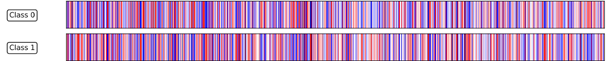
\includegraphics[scale=0.6]{images/weights_voice_qt}
		\end{figure}
		\vspace*{4mm}
		\item Red bars indicate high weights, blue bars indicate low values, white / light bars represent weights around zero.
		\item $\Rightarrow$ It might be useful to add a threshold.
	\end{itemize}
\end{frame}


% Embedding Projections
\begin{frame}{Embedding Projections}{}
	\vspace*{-4mm}
	\begin{figure}
		\centering
		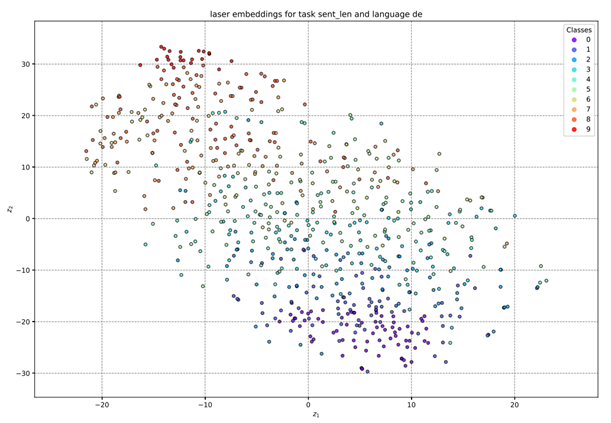
\includegraphics[scale=0.5]{images/scatter_sent_len_laser}
	\end{figure}
\end{frame}


% Confusion Matrix
\begin{frame}{Confusion Matrix}{}
	\vspace*{-4mm}
	\begin{itemize}
		\item Confusion matrix for task \textit{`sentence length'}, \textit{`LASER'} embeddings and language \textit{`de'}:
	\end{itemize}

	\begin{figure}
		\centering
		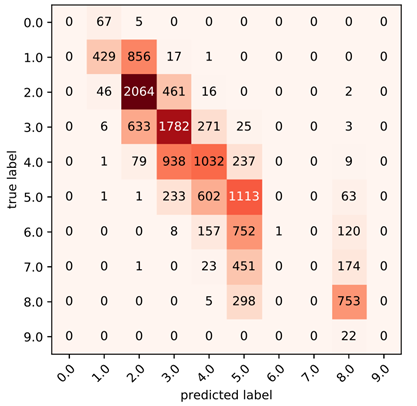
\includegraphics[scale=0.45]{images/conf_mat_sent_len_laser}
	\end{figure}
\end{frame}

\end{document}
